\title{Midterm 2 for Algebra-Based Physics: Electricity and Magnetism}
\author{Dr. Jordan Hanson - Whittier College Dept. of Physics and Astronomy}
\date{\today}
\documentclass[10pt]{article}
\usepackage[a4paper, total={18cm, 27cm}]{geometry}
\usepackage{outlines}
\usepackage{graphicx}
\begin{document}
\maketitle

\section{Equations and constants}

\begin{enumerate}
\item Kirchhoff's Rules: 1) $I_{in} + I_{out} = 0$ (Junction Rule) 2) $\sum_{loop} V_i = 0$ (Loop Rule)
\item Ohm's Law: $V = IR$
\item Power from current: $P=IV$
\item Voltage in an RC across the capacitor: $V(t) = \epsilon\left(1 - \exp\left(-t/\tau\right)\right)$, where $\epsilon$ is the battery voltage and the time constant is $\tau = RC$.
\item Centripetal force: $F_C = mv^2/r$.
\item Magnetic torque: $\vec{\tau}_B = \vec{\mu} \times \vec{B}$
\item Magnitude of torque: $|\vec{\tau}_B| = \mu B \sin\theta$
\item Magnetic dipole moment: $\vec{\mu} = I \vec{A}$ (the current times the area vector)
\item Magnetic field at the center of a current-carrying loop: $\vec{B} = (\mu_0 I)/(2 R)\hat{z}$, if the current is in the x-y plane.
\item Magnetic field due to a \textbf{long straight wire} at a distance R: $B = (\mu_0 I)/(2 \pi R)$, right-hand rule gives direction.
\item Ampere's Law: $\int \vec{B} \cdot d\vec{s} = \mu_0 I_{enc}$ which is $B S = \mu_0 I_{enc}$ for simple cases where B is constant around the path.
\item Magnetic permeability: $\mu_0 = 4\pi \times 10^{-7}$ T m A$^{-1}$
\item The Hall Effect: $V_H = B l v$.
\item Charge of an electron/proton: $q_e = 1.6 \times 10^{-19}$ C.
\item Mass of proton: $1.67 \times 10^{-27}$ kg.
\end{enumerate}

\clearpage

\section{Exercises}

\begin{enumerate}
\item \textbf{Chapter 21: DC Circuits and Kirchhoff's Rules}
\begin{enumerate}
\item 
\begin{figure}[ht]
\centering
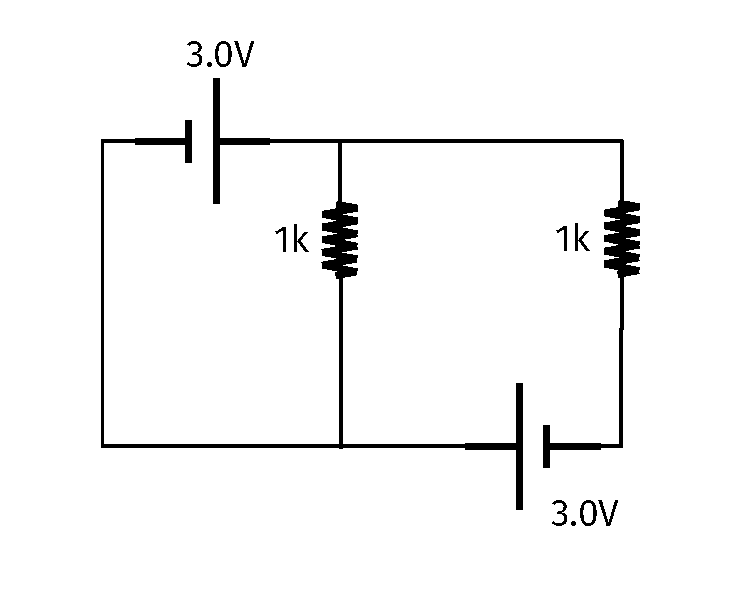
\includegraphics[width=0.5\textwidth]{iV.pdf}
\caption{\label{fig:circuit1} A circuit with three resistors powered by two voltages.}
\end{figure}
What are the currents flowing through each resistor in Fig. \ref{fig:circuit1}? \textit{Hint: first define the current in each segment of the circuit.  Then apply the junction rule once and the loop rule twice.}\\ \vspace{10cm}
\item An RC circuit has a time constant $\tau = 1$ ms.  If the resistance is $R = 1$ k$\Omega$, what is the value of the capacitor? \\ \vspace{1cm}
\end{enumerate}
\item \textbf{Chapter 22: Magnetic fields}
\begin{enumerate}
\item What Hall voltage is produced by a 0.1 T field applied across a 5 mm diamter blood vessel when blood velocity is 90.0 cm/s? \\ \vspace{1cm}
\item (a) An iron ion with a mass of $9.28\times 10^{-26}$ kg travels at $2.00 \times 10^{6}$ m/s perpendicular to a 1.0 T magnetic field, which makes it move in a circular path. If it is singly-ionized, it has the charge of $q_e = 1.6 \times 10^{-19}$ C. (a) What is the radius of the circular path it traverses? (b) What would happen to the radius of the path if the B-field value was slowly increased? \\ \vspace{2cm}
\item Determine the direction of the Lorentz force in each of the following cases:
\begin{enumerate}
\item B-field is to the right, velocity of positively charged particle is up:
\item B-field is out of the page, velocity of positively charged particle to the left:
\item B-field is to the right, velocity of negatively charged particle is down:
\end{enumerate} \vspace{0.2cm}
\item Determine the direction of the velocity of the charge in each of the following cases:
\begin{enumerate}
\item B-field is to the right, force of positively charged particle is up:
\item B-field is out of the page, force of positively charged particle to the right:
\item B-field is down, force of negatively charged particle is out of page:
\end{enumerate} \vspace{0.2cm}
\item What is the (a) maximum torque on a 200-turn circular loop of wire with radius 4.0 cm that carries a 10.0-A current in a 0.5 T B-field? (b) What is the magnetic moment of this object? \\ \vspace{2 cm}
\item Model an arch of electricity from a faulty transformer to the wooden pole holding it as a \textbf{long straight wire}.  A typical current is $30.0$ A. (a) Estimate the magnetic field 1 m from the arch of electricity. (b) How does the result compare to the magnetic field of the Earth at the ground ($\approx 0.5$ Gauss)? \\ \vspace{1cm}
\item 
\begin{figure}[hb]
\centering
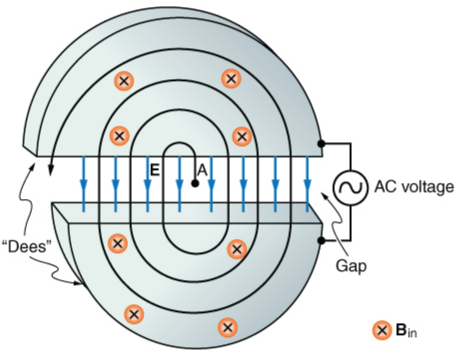
\includegraphics[width=0.3\textwidth]{cyclo.png}
\caption{\label{fig:cyclo} Each diagram depicts the force on a positively-charged particle in a B-field.}
\end{figure}
The period $T$ of the circular orbit of a charged particle with mass $m$ and charge $q$ moving perpendicularly to a uniform magnetic field is $T = 2\pi m/(qB)$. (a) What is the frequency $f = T^{-1}$ at which protons circulate as shown in Fig. \ref{fig:cyclo}? Assume the B-field is 2.0 T and the charge and mass of protons are given in the equations list.  (b) What is the frequency for alpha particles?  (The mass of an alpha is 4 times the mass of a proton, and the charge is twice that of a proton - think of this as a scaling problem).
\end{enumerate}
\end{enumerate}
\end{document}